\documentclass[11pt,a4paper]{article}
\usepackage[T1]{fontenc}
\usepackage[utf8]{inputenc}
\usepackage[french]{babel}
\usepackage[margin=2.4cm]{geometry}
\usepackage{amsmath}
\usepackage{amssymb}
\usepackage{graphicx}
\usepackage{booktabs}
\usepackage{xcolor}
\usepackage{caption}
\usepackage[hidelinks]{hyperref}
\graphicspath{{../figures/}}
\captionsetup{font=small,labelfont=bf}

% ==== BEGIN RESULTS (valeurs injectées depuis results.json par inject_results.py) ====
\newcommand{\accLogReg}{0{,}00}
\newcommand{\fLogReg}{0{,}00}
\newcommand{\accMLP}{0{,}00}
\newcommand{\fMLP}{0{,}00}
\newcommand{\accCNN}{0{,}00}
\newcommand{\fCNN}{0{,}00}
\newcommand{\accResnet}{0{,}00}
\newcommand{\fResnet}{0{,}00}
\newcommand{\bestlr}{1\times10^{-3}}
\newcommand{\cnnparams}{1\,440\,298}
\newcommand{\bestclass}{--}
\newcommand{\worstclass}{--}
\newcommand{\ablbase}{0{,}00}
\newcommand{\ablnoaug}{0{,}00}
\newcommand{\ablnobn}{0{,}00}
% ==== END RESULTS ====

\newcommand{\code}[1]{\texttt{#1}}

\title{Classification morphologique de galaxies par réseau de neurones convolutif\\
\large Galaxy10 DECaLS : baselines, CNN maison, transfer learning et Grad-CAM}
\author{Patrick Yvan Eyike \and Philémon Vittet \and Sidi Hamadi \and
Abdelrahman Dahy \and Inès Lylia Zerdani}
\date{Juillet 2026}

\begin{document}
\maketitle

\begin{abstract}
\noindent
On classe la morphologie de 17\,736 galaxies du relevé DESI Legacy Imaging Surveys
(dataset Galaxy10 DECaLS, labels Galaxy Zoo) en 10 classes, à l'aide d'un réseau
convolutif. Pour isoler l'apport de la convolution, on compare trois niveaux :
baselines sans convolution (régression logistique, MLP), un CNN maison de
\cnnparams{} paramètres, et un ResNet18 pré-entraîné sur ImageNet. Le meilleur modèle
atteint une accuracy de \accResnet{} et un F1 macro de \fResnet{} sur le test officiel.
On interprète les prédictions par Grad-CAM et on quantifie l'apport de l'augmentation
et de la BatchNorm par ablation. Le rapport insiste sur un point de fond : l'équivariance
par translation du CNN est une symétrie imposée à l'architecture, dans l'esprit des
symétries en physique.
\end{abstract}

\section{Introduction et contexte}

La morphologie d'une galaxie (spirale, elliptique, barrée, en fusion) porte une
information physique : elle est liée à l'histoire de formation, à l'environnement et à
la dynamique du système. À l'échelle des grands relevés, trier des millions de galaxies
à la main est impossible. Le projet Galaxy Zoo a mobilisé des centaines de milliers de
volontaires pour labelliser des images ; c'est de là que viennent nos étiquettes. La
question de ce projet est simple : un réseau convolutif peut-il reproduire ce tri
morphologique de façon automatique et fiable ?

On répond en construisant une échelle de trois modèles de complexité croissante, de la
baseline aveugle à la structure spatiale jusqu'au réseau pré-entraîné, puis en
interprétant ce que le réseau a appris. Historiquement, cette famille de modèles remonte
à LeNet (LeCun, 1998), premier CNN entraîné par rétropropagation pour la lecture de
chiffres, et à AlexNet (Krizhevsky, 2012), qui a démontré à grande échelle sur ImageNet
la supériorité des CNN profonds et relancé tout le domaine.

\section{Données}

Galaxy10 DECaLS contient 17\,736 images couleur $256\times256$ (bandes $g$, $r$, $z$ du
relevé DESI Legacy Imaging Surveys), réparties en 10 classes morphologiques. Le
tableau~\ref{tab:classes} donne les effectifs : la distribution est fortement
déséquilibrée, d'un facteur proche de 8 entre la classe la plus rare (Cigar Shaped, 334
images) et la plus fréquente (Round Smooth, 2\,645). Ce déséquilibre est un point central
de l'évaluation.

\begin{table}[h]
\centering
\small
\begin{tabular}{clr@{\qquad}clr}
\toprule
id & classe & $n$ & id & classe & $n$ \\
\midrule
0 & Disturbed & 1\,081 & 5 & Barred Spiral & 2\,043 \\
1 & Merging & 1\,853 & 6 & Unbarred Tight Spiral & 1\,829 \\
2 & Round Smooth & 2\,645 & 7 & Unbarred Loose Spiral & 2\,628 \\
3 & In-between Round Smooth & 2\,027 & 8 & Edge-on without Bulge & 1\,423 \\
4 & Cigar Shaped Smooth & 334 & 9 & Edge-on with Bulge & 1\,873 \\
\bottomrule
\end{tabular}
\caption{Les 10 classes de Galaxy10 DECaLS et leurs effectifs.}
\label{tab:classes}
\end{table}

\begin{figure}[h]
\centering
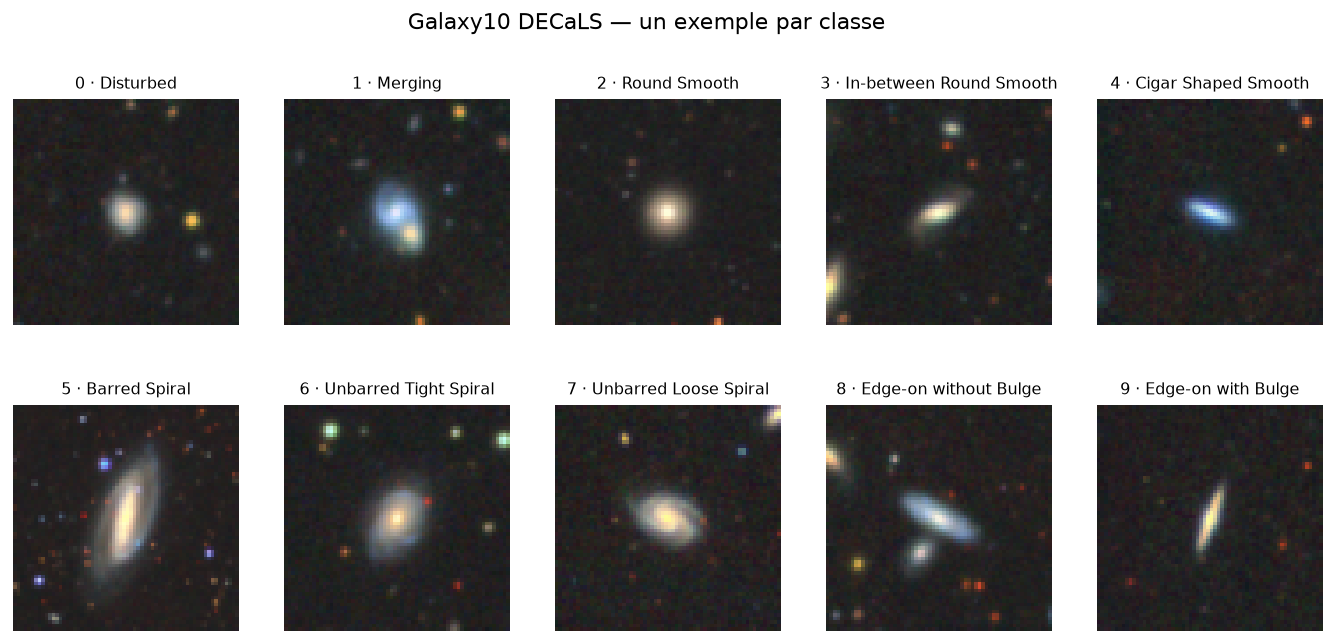
\includegraphics[width=\textwidth]{samples.png}
\caption{Un exemple par classe. Les classes voisines sont visuellement proches :
spirales serrées contre lâches, rondes contre cigare, edge-on avec ou sans bulbe.}
\label{fig:samples}
\end{figure}

\paragraph{Découpage.} Le dataset fournit déjà un \code{train} (16\,000) et un
\code{test} (1\,800). On garde le test officiel comme test final, jamais utilisé pendant
le développement, et on tire une validation stratifiée de 15\,\% dans le train (seed
figé). Toutes les décisions (choix de modèle, hyperparamètres) se prennent sur la
validation. Ce protocole évite deux fuites classiques : décider sur le test, et augmenter
les données avant le découpage.

\section{Éléments de théorie}

\subsection{Du perceptron au réseau profond}

Un réseau de neurones enchaîne des couches affines $z = Wx + b$ suivies d'une
non-linéarité, typiquement la ReLU $\sigma(z)=\max(0,z)$. La dernière couche produit un
vecteur de scores transformé en probabilités par la softmax
$p_k = e^{z_k} / \sum_j e^{z_j}$. On entraîne en minimisant l'entropie croisée
\begin{equation}
\mathcal{L} = -\sum_{k} y_k \log p_k = -\log p_{y},
\end{equation}
qui n'est autre que la log-vraisemblance négative du bon label sous le modèle : minimiser
l'entropie croisée revient à maximiser la vraisemblance des données. Les gradients se
calculent par rétropropagation (application organisée de la règle de la chaîne, de la
loss vers les poids), et on met à jour les paramètres par descente de gradient
stochastique ou, ici, par Adam. Le learning rate est l'hyperparamètre le plus sensible :
trop grand, la loss diverge ; trop petit, rien n'apprend.

\subsection{La convolution 2D}

Une couche convolutive fait glisser un même petit filtre sur toute l'image et calcule, en
chaque position, une somme pondérée locale :
\begin{equation}
(I * K)_{i,j} = \sum_{m}\sum_{n} I_{i+m,\,j+n}\, K_{m,n}.
\end{equation}
C'est exactement la convolution discrète familière en traitement du signal, le filtre
jouant le rôle de réponse impulsionnelle : chaque canal de sortie est un détecteur d'un
motif local (bord, tache, orientation). Deux propriétés en découlent.

\emph{Partage de poids.} Le même filtre sert partout dans l'image. Le nombre de paramètres
ne dépend donc pas de la taille de l'image mais seulement de la taille du filtre et du
nombre de canaux, ce qui rend l'apprentissage statistiquement efficace et régularise le
modèle.

\begin{center}
\fbox{\parbox{0.93\textwidth}{
\textbf{Équivariance par translation et symétries.} Comme le filtre est appliqué de façon
identique partout, translater un motif dans l'image translate d'autant sa réponse :
$f(T_v\,x) = T_v\,f(x)$. Le CNN encode donc \emph{a priori} une symétrie du problème dans
son architecture, plutôt que de devoir l'apprendre. C'est le même principe qu'en physique,
où l'on impose les symétries d'un système (invariances par translation, rotation) avant de
résoudre les équations. Une galaxie n'ayant pas de position ni d'orientation privilégiée
dans le ciel, ces invariances sont physiquement justifiées, et l'on complète l'équivariance
par translation du CNN avec une augmentation par rotations et symétries (section~4).
}}
\end{center}

\subsection{Architecture et champ réceptif}

On empile des blocs \code{Conv $\to$ BatchNorm $\to$ ReLU $\to$ MaxPool}. Le pooling réduit
la résolution spatiale et augmente le champ réceptif : les couches profondes voient une
portion de plus en plus grande de l'image d'origine, ce qui construit une hiérarchie de
features, des bords locaux aux textures puis aux formes globales (bras spiraux, barre,
compagnon de fusion).

\subsection{Dimensionnement et nombre de paramètres}

Notre CNN prend une entrée $3\times64\times64$. Une convolution $3\times3$ avec padding 1
conserve la taille spatiale ; chaque MaxPool la divise par deux. Le
tableau~\ref{tab:dims} suit les dimensions bloc par bloc.

\begin{table}[h]
\centering
\small
\begin{tabular}{lcc}
\toprule
couche & sortie $(C,H,W)$ & poids conv (sans biais) \\
\midrule
entrée & $3\times64\times64$ & -- \\
bloc 1 : Conv$(3\to32)$+pool & $32\times32\times32$ & $3\cdot32\cdot9 = 864$ \\
bloc 2 : Conv$(32\to64)$+pool & $64\times16\times16$ & $32\cdot64\cdot9 = 18\,432$ \\
bloc 3 : Conv$(64\to128)$+pool & $128\times8\times8$ & $64\cdot128\cdot9 = 73\,728$ \\
bloc 4 : Conv$(128\to256)$+pool & $256\times4\times4$ & $128\cdot256\cdot9 = 294\,912$ \\
AdaptiveAvgPool$(4\times4)$ & $256\times4\times4$ & -- \\
FC $4096\to256$ & 256 & $4096\cdot256+256 = 1\,048\,832$ \\
FC $256\to10$ & 10 & $256\cdot10+10 = 2\,570$ \\
\bottomrule
\end{tabular}
\caption{Dimensions et paramètres du CNN maison. Les convolutions sont sans biais (la
BatchNorm fournit le décalage). En ajoutant les $2$ paramètres par canal de BatchNorm
($64+128+256+512 = 960$), le total est de \cnnparams{} paramètres, dominé à 73\,\% par la
première couche dense. L'\code{AdaptiveAvgPool} fixe la taille de la tête, ce qui garde ce
compte identique en 64 comme en 128 px.}
\label{tab:dims}
\end{table}

\subsection{Régularisation}

Un réseau à plus d'un million de paramètres sur quelques milliers d'images sur-apprend
facilement. On combine trois régularisations. Le \emph{dropout} éteint aléatoirement des
unités pendant l'entraînement. La \emph{BatchNorm} normalise les activations par mini-lot,
ce qui stabilise et accélère l'apprentissage. La \emph{data augmentation} enrichit
artificiellement le train avec des transformations qui préservent le label : ici rotations
0--360$^\circ$, symétries horizontales et verticales, léger jitter de luminosité. Comme
souligné plus haut, ces transformations sont des invariances physiques du problème et non
un simple bruit.

\subsection{Transfer learning}

Plutôt que d'apprendre de zéro, on réutilise un ResNet18 pré-entraîné sur ImageNet. Le
ResNet introduit les connexions résiduelles $y = \mathcal{F}(x)+x$, qui laissent le
gradient circuler et permettent d'entraîner des réseaux profonds. On remplace la dernière
couche par 10 sorties et on procède en deux temps : \emph{feature extraction} (backbone
gelé, on n'entraîne que la tête) puis \emph{fine-tuning} (tout dégelé, learning rate plus
faible).

\section{Pipeline expérimental}

Les images sont redimensionnées en 64 px (baselines et CNN) et 128 px (ResNet), puis
normalisées canal par canal avec des statistiques calculées \emph{sur le train
uniquement}. L'augmentation n'est appliquée qu'au train, jamais à la validation ni au
test. Le déséquilibre est traité en pondérant l'entropie croisée par l'inverse des
fréquences de classe, et l'évaluation privilégie le F1 macro (qui traite toutes les
classes à égalité) plutôt que la seule accuracy. L'entraînement utilise Adam, un scheduler
cosine et un early stopping sur le F1 macro de validation. Le code est organisé en un
package Python réutilisable et un notebook auto-portant ; les runs tournent indifféremment
en local (Mac, backend MPS) et sur Colab (GPU T4), avec détection automatique du device.

\section{Expériences et résultats}

\subsection{L'échelle baseline $\to$ CNN $\to$ ResNet}

Le tableau~\ref{tab:scale} et la figure~\ref{fig:echelle} résument l'apport de la
convolution. Les baselines, aveugles à la structure spatiale, restent médiocres. Le CNN
maison progresse nettement, et le transfer learning ajoute encore un cran.

\begin{table}[h]
\centering
\small
\begin{tabular}{lcc}
\toprule
modèle & accuracy & F1 macro \\
\midrule
Régression logistique (pixels) & \accLogReg & \fLogReg \\
MLP 2 couches (pixels) & \accMLP & \fMLP \\
CNN maison & \accCNN & \fCNN \\
ResNet18 (fine-tuné) & \accResnet & \fResnet \\
\bottomrule
\end{tabular}
\caption{Performances sur le test officiel (jamais utilisé pendant le développement).}
\label{tab:scale}
\end{table}

\begin{figure}[h]
\centering
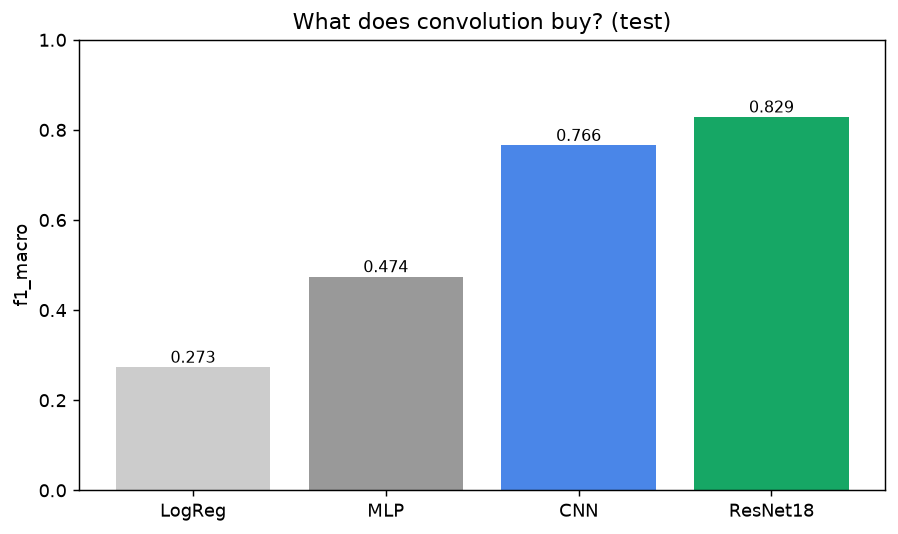
\includegraphics[width=0.72\textwidth]{echelle.png}
\caption{F1 macro sur le test, des baselines au ResNet. La convolution, puis le
pré-entraînement, expliquent l'essentiel du gain.}
\label{fig:echelle}
\end{figure}

\subsection{Tuning et courbes d'apprentissage}

Le learning rate est réglé sur la validation ; la meilleure valeur est
$\text{lr}=\bestlr$. Les courbes de la figure~\ref{fig:courbes} montrent l'évolution de la
loss et du F1 macro de validation, avec l'epoch retenue par early stopping.

\begin{figure}[h]
\centering
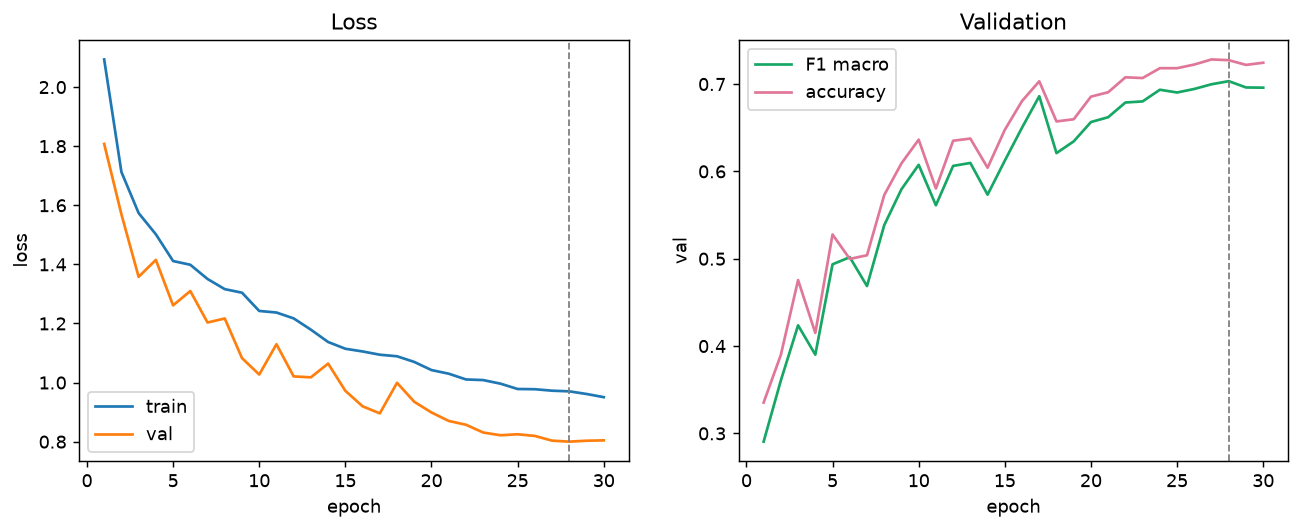
\includegraphics[width=\textwidth]{courbes.png}
\caption{Courbes d'apprentissage du CNN maison (loss train/val et métriques de
validation). La ligne verticale marque l'epoch du meilleur F1 macro.}
\label{fig:courbes}
\end{figure}

\subsection{Analyse par classe et confusions}

La matrice de confusion (figure~\ref{fig:confusion}) et le F1 par classe
(figure~\ref{fig:perclass}) montrent où le modèle se trompe. Les erreurs se concentrent
sans surprise entre classes morphologiquement voisines. La classe \bestclass{} est la
mieux reconnue ; la classe \worstclass{} reste la plus difficile, ce qui est cohérent avec
son faible effectif et son ambiguïté visuelle.

\begin{figure}[h]
\centering
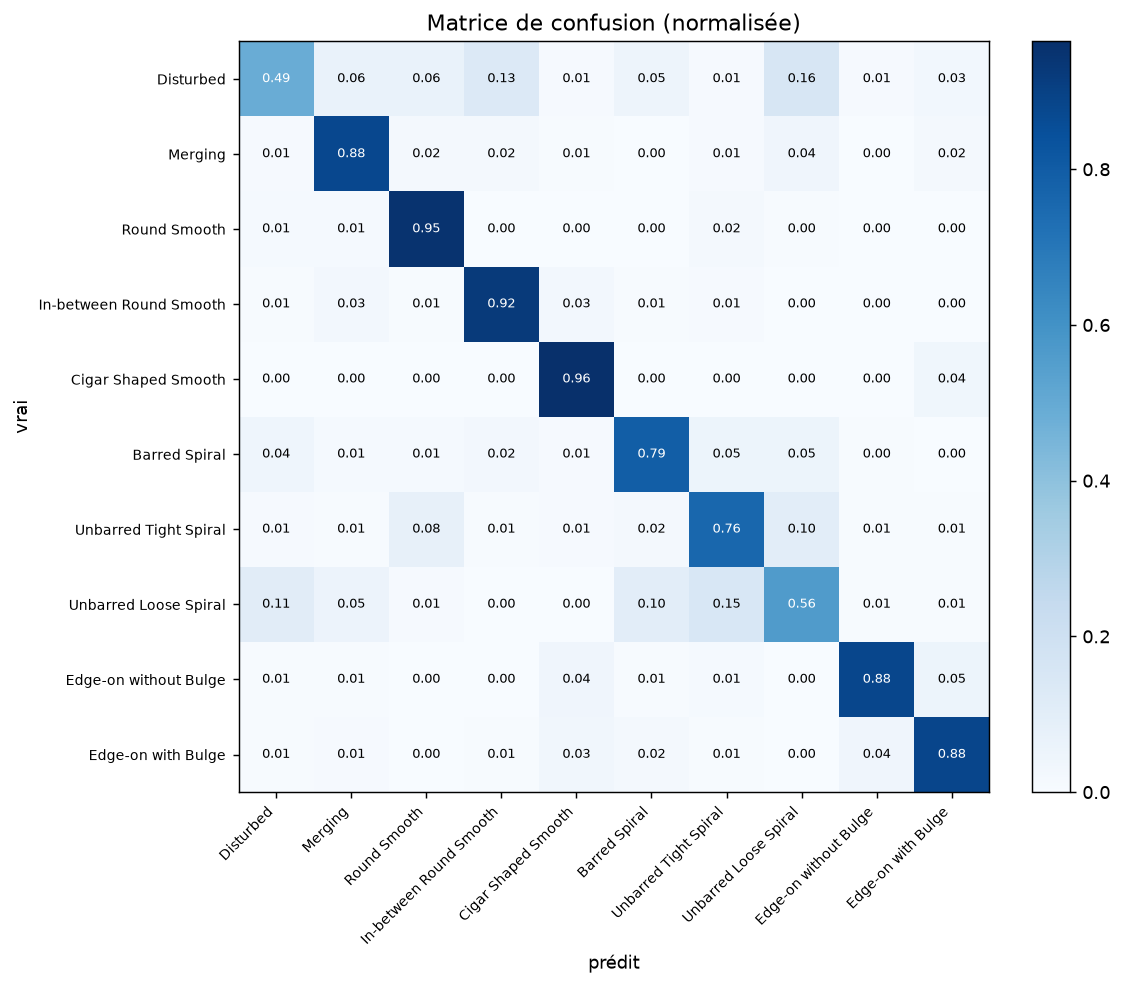
\includegraphics[width=0.7\textwidth]{confusion.png}
\caption{Matrice de confusion normalisée par ligne (ResNet18, test).}
\label{fig:confusion}
\end{figure}

\begin{figure}[h]
\centering
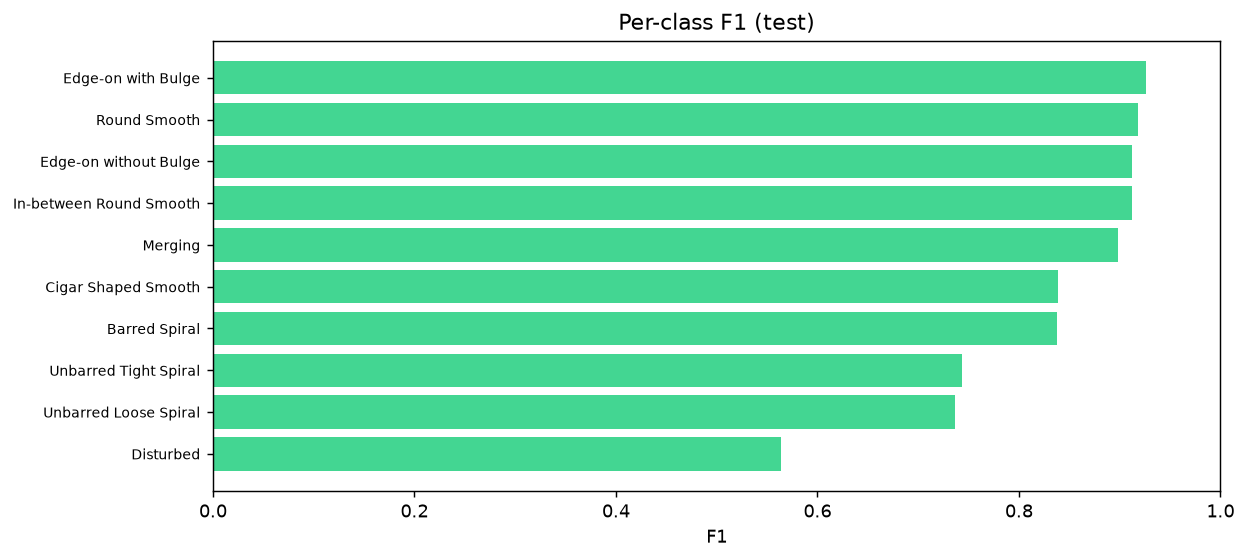
\includegraphics[width=0.8\textwidth]{perclass.png}
\caption{F1 par classe sur le test. Les classes rares et ambiguës sont en bas.}
\label{fig:perclass}
\end{figure}

\subsection{Interprétation par Grad-CAM}

Grad-CAM pondère les feature maps de la dernière convolution par le gradient moyen du
score de la classe, applique une ReLU, puis rééchelonne à la taille de l'image ; on obtient
une carte de chaleur des régions qui pilotent la prédiction. La
figure~\ref{fig:gradcam} montre des cas corrects et des erreurs. Sur les bonnes
prédictions, le réseau se concentre sur les structures pertinentes (bras spiraux, barre,
compagnon de fusion) ; sur les erreurs, la carte révèle parfois un appui sur un objet
voisin ou un artefact.

\begin{figure}[h]
\centering
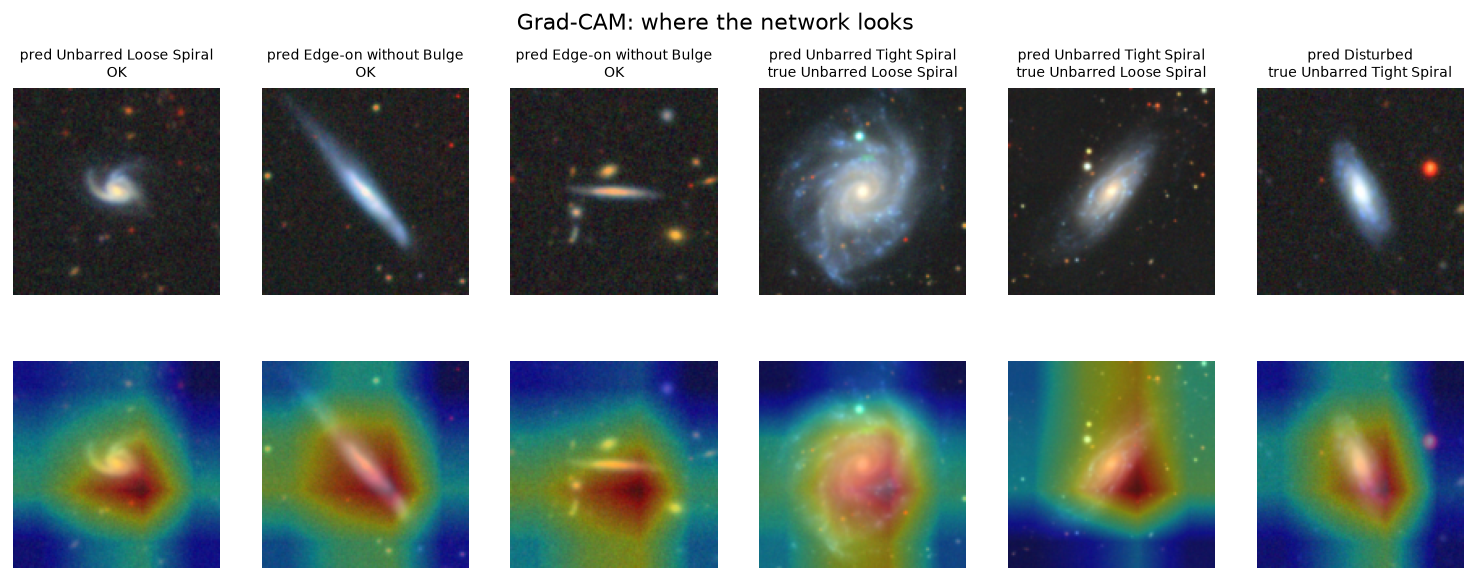
\includegraphics[width=\textwidth]{gradcam_resnet.png}
\caption{Grad-CAM sur le ResNet18 (ligne haute : image ; ligne basse : carte superposée).
Prédictions correctes puis erreurs.}
\label{fig:gradcam}
\end{figure}

\subsection{Ablations}

On retire un ingrédient à la fois pour mesurer son apport (F1 macro sur le test). Le CNN
complet atteint \ablbase{} ; sans augmentation il tombe à \ablnoaug{}, et sans BatchNorm à
\ablnobn{}. Chaque composant contribue donc mesurablement à la performance et à la
stabilité de l'entraînement.

\begin{figure}[h]
\centering
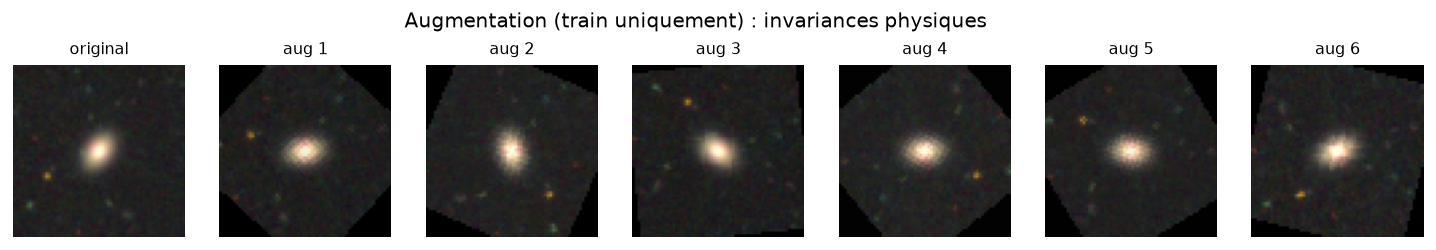
\includegraphics[width=0.85\textwidth]{augment.png}
\caption{Effet de l'augmentation sur une même galaxie (rotations, symétries, jitter). Le
label est préservé, l'apparence varie.}
\label{fig:augment}
\end{figure}

\section{Limites}

Trois limites principales. Les labels de Galaxy Zoo sont bruités : ils agrègent des votes
de volontaires et les frontières entre classes voisines sont floues, ce qui plafonne
mécaniquement la performance atteignable. Le déséquilibre pénalise les classes rares
malgré la pondération de la loss. Enfin, le coût d'entraînement limite l'exploration : on a
travaillé en 64 et 128 px plutôt qu'en 256, et l'espace des hyperparamètres n'a été
balayé que partiellement.

\section{Conclusion}

L'échelle baseline $\to$ CNN $\to$ ResNet répond à la question de départ : la convolution,
puis le transfer learning, apportent l'essentiel de la performance, et le meilleur modèle
reproduit correctement le tri morphologique de Galaxy Zoo. Grad-CAM confirme que le réseau
s'appuie sur les structures morphologiques attendues, et les ablations quantifient l'apport
de chaque ingrédient. Le point conceptuel à retenir est que le succès du CNN sur des images
tient largement à une symétrie imposée par construction, l'équivariance par translation,
prolongée par une augmentation qui encode les invariances physiques du problème.

\end{document}
